\documentclass[
    crop,
    tikz
    ]{standalone}

\begin{document}

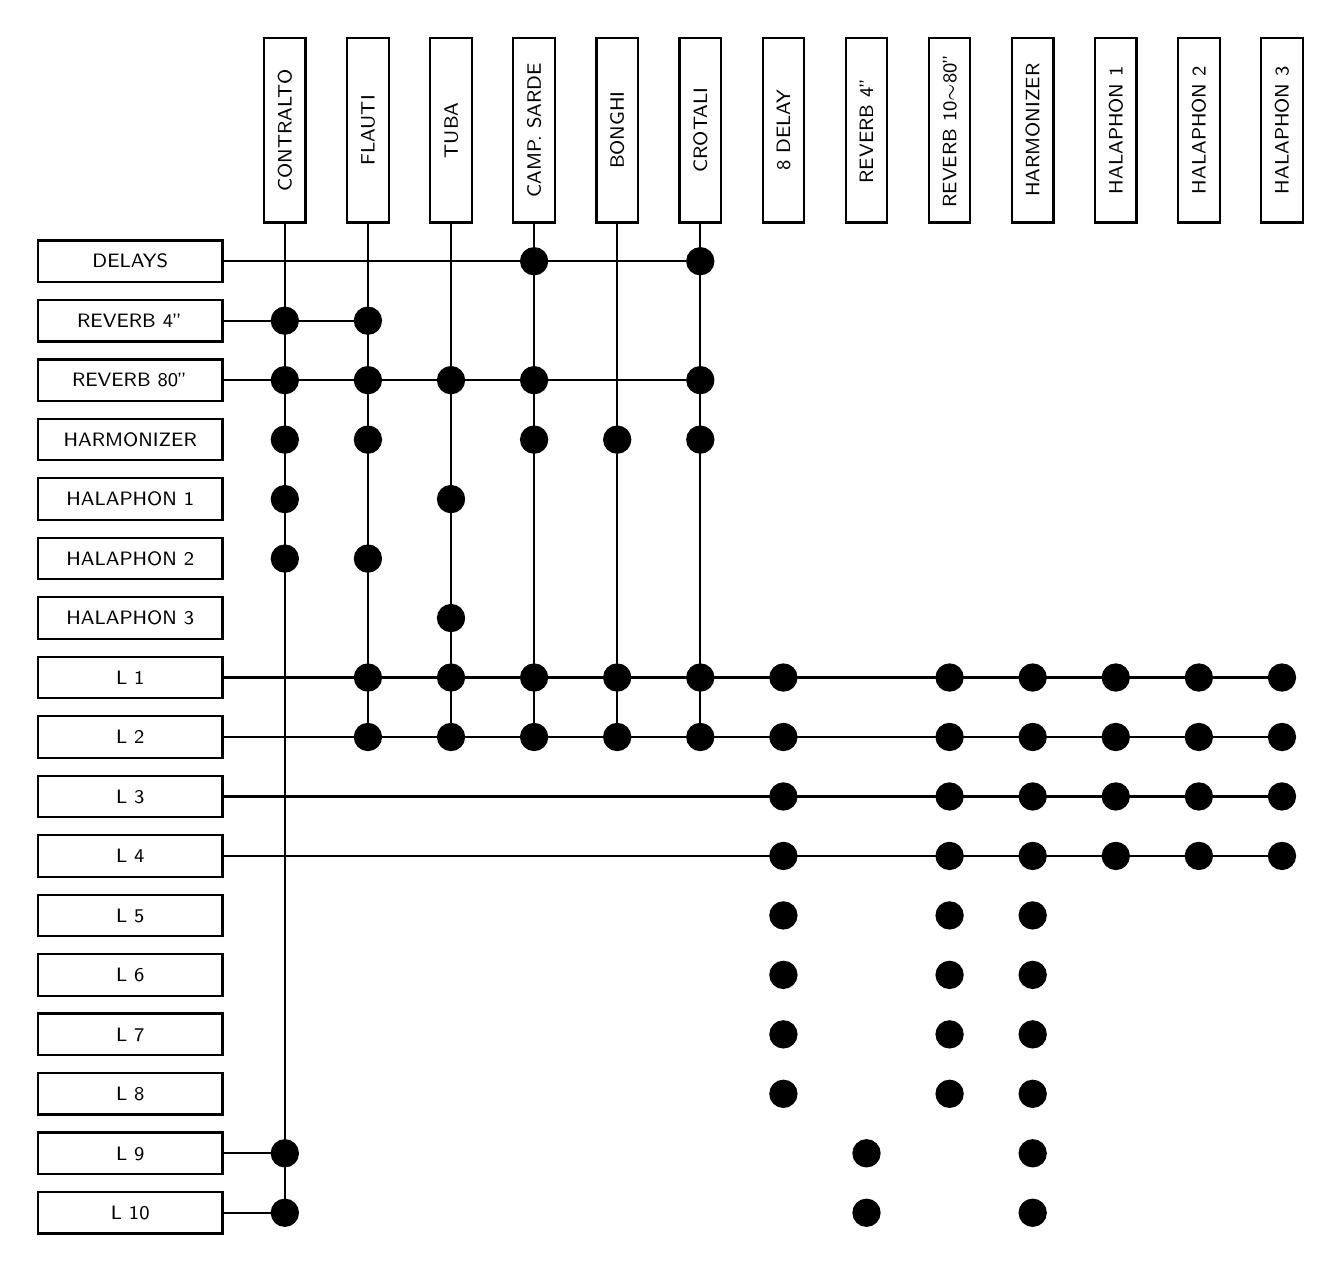
\begin{tikzpicture}[
    %auto,
    inputs/.style    = {
    	font=\scriptsize\sffamily,
    	rectangle,
		draw=black,
		thick,
		%fill=black!10,
		text width=6em,
		text centered,
		%rounded corners,
		minimum height=1.5em,
		rotate=90
		},
    outs/.style    = {
    	font=\scriptsize\sffamily,
    	rectangle,
		draw=black,
		thick,
		%fill=black!10,
		text width=6em,
		text centered,
		%rounded corners,
		minimum height=1.5em,
		%rotate=-90
		},
	line/.style = {
    	draw,
		thick,
		fill=black
		%shorten >=2pt
		},
	ctl/.style = {
    	draw,
		circle,
		thick,
		fill=black,
		%shorten >=2pt
		},
empty/.style = {
		},
    arrow/.style = {
    	draw,
		thick,
		->,
		shorten >=2pt
		},
  ]
  % Define nodes in a matrix
\matrix [column sep=5mm, row sep=2mm]{
	& \node [inputs] (c)  {CONTRALTO};
	& \node [inputs] (fl) {FLAUTI};
	& \node [inputs] (tb) {TUBA};
  & \node [inputs] (cs) {CAMP. SARDE};
	& \node [inputs] (bng) {BONGHI};
	& \node [inputs] (crt) {CROTALI};
	& \node [inputs] (dly) {8 DELAY};
	& \node [inputs] (r4) {REVERB 4"};
	& \node [inputs] (r80) {REVERB 10$\sim$80"};
	& \node [inputs] (har) {HARMONIZER};
	& \node [inputs] (h1) {HALAPHON 1};
	& \node [inputs] (h2) {HALAPHON 2};
	& \node [inputs] (h3) {HALAPHON 3}; \\
	% -------------------------------&---------------------&--------------------&--------------------&--------------------&--------------------&-----------------&-----------------&-----------------&-----------------&-----------------&-----------------&-----------------&-----------------
  % -------------------------------&--CONTRALTO----------&--FLAUTO------------&--TUBA--------------&--CAMPANE-SARDE-----&--BONGOS-------------&--CROTALI------------&--DELAY----------&--REV4-----------&--REV80----------&--HARMONIZER-----&--HALAPHON 1-----&--HALAPHON 2-----&--HALAPHON 3-----
	\node [outs] (dly) {DELAYS};     &                     &                    &                    & \node[ctl](){};    &                     & \node[ctl](crtdly){};     &                 &                 &                 &                 &                 &                 &  \\
	\node [outs] (r4) {REVERB 4"};   & \node[ctl](){};     & \node[ctl](flr4){};&                    &                    &                     &                     &                 &                 &                 &                 &                 &                 &  \\
	\node [outs] (r80) {REVERB 80"}; & \node[ctl](){};     & \node[ctl](){};    & \node[ctl](){};    & \node[ctl](){};    &                     & \node[ctl](crtr80){};&                 &                 &                 &                 &                 &                 &  \\
	\node [outs] (har) {HARMONIZER}; & \node[ctl](){};     & \node[ctl](){};    &                    & \node[ctl](){};    & \node[ctl](){};     & \node[ctl](){};     &                 &                 &                 &                 &                 &                 &  \\
	\node [outs] (h1) {HALAPHON 1};  & \node[ctl](){};     &                    & \node[ctl](){};    &                    &                     &                     &                 &                 &                 &                 &                 &                 &  \\
	\node [outs] (h2) {HALAPHON 2};  & \node[ctl](){};     & \node[ctl](){};    &                    &                    &                     &                     &                 &                 &                 &                 &                 &                 &  \\
	\node [outs] (h3) {HALAPHON 3};  &                     &                    & \node[ctl](){};    &                    &                     &                     &                 &                 &                 &                 &                 &                 &  \\
	\node [outs] (l1) {L 1};         &                     & \node[ctl](){};    & \node[ctl](){};    & \node[ctl](){};    & \node[ctl](){};     & \node[ctl](){};     & \node[ctl](){}; &                 & \node[ctl](){}; & \node[ctl](){}; & \node[ctl](){}; & \node[ctl](){}; & \node[ctl](h3l1){}; \\
	\node [outs] (l2) {L 2};         &                     & \node[ctl](fl2){}; & \node[ctl](tb2){}; & \node[ctl](cs2){}; & \node[ctl](bng2){}; & \node[ctl](crt2){}; & \node[ctl](){}; &                 & \node[ctl](){}; & \node[ctl](){}; & \node[ctl](){}; & \node[ctl](){}; & \node[ctl](h3l2){}; \\
	\node [outs] (l3) {L 3};         &                     &                    &                    &                    &                     &                     & \node[ctl](){}; &                 & \node[ctl](){}; & \node[ctl](){}; & \node[ctl](){}; & \node[ctl](){}; & \node[ctl](h3l3){}; \\
	\node [outs] (l4) {L 4};         &                     &                    &                    &                    &                     &                     & \node[ctl](){}; &                 & \node[ctl](){}; & \node[ctl](){}; & \node[ctl](){}; & \node[ctl](){}; & \node[ctl](h3l4){}; \\
	\node [outs] (l5) {L 5};         &                     &                    &                    &                    &                     &                     & \node[ctl](){}; &                 & \node[ctl](){}; & \node[ctl](){}; &                 &                 &  \\
	\node [outs] (l6) {L 6};         &                     &                    &                    &                    &                     &                     & \node[ctl](){}; &                 & \node[ctl](){}; & \node[ctl](){}; &                 &                 &  \\
	\node [outs] (l7) {L 7};         &                     &                    &                    &                    &                     &                     & \node[ctl](){}; &                 & \node[ctl](){}; & \node[ctl](){}; &                 &                 &  \\
	\node [outs] (l8) {L 8};         &                     &                    &                    &                    &                     &                     & \node[ctl](){}; &                 & \node[ctl](){}; & \node[ctl](){}; &                 &                 &  \\
	\node [outs] (l9) {L 9};         & \node[ctl](cl9){};  &                    &                    &                    &                     &                     &                 & \node[ctl](){}; &                 & \node[ctl](){}; &                 &                 &  \\
	\node [outs] (l10) {L 10};       & \node[ctl](cl10){}; &                    &                    &                    &                     &                     &                 & \node[ctl](){}; &                 & \node[ctl](){}; &                 &                 &  \\
};

%	& \node [draw,circle] (inputs) {+}; & & & \node [draw,circle] (direct) {+}; & \\
%	& \node[ctl](){}; & & \node [block] (victor) {VICTOR}; & \node [draw,circle] (mix1) {+}; & \\
%	& \node [ctl] (node2) {}; & & \node [block] (freezer) {FREEZER}; & \node [draw,circle] (mix2) {+}; & \\
%	& \node [ctl] (node3) {}; & & \node [block] (sdelay) {SPECTRAL DELAY}; & \node [draw,circle] (mix3) {+}; & \\
%	& & & \node [block] (bfmt) {B-FORMAT}; & \node [block] (afmt) {A-FORMAT}; & \\
%	& & & \node [block] (outputs) {STEREO / QUAD}; & \node [block] (stone) {S.T.ONE}; & \\


\begin{scope} [every path/.style=line]
  \path (dly) -- (crtdly);
  \path (r4) -- (flr4);
  \path (r80) -- (crtr80);
  \path (c) -- (cl10);
  \path (l9) -- (cl9);
  \path (l10) -- (cl10);
  \path (fl) -- (fl2);
  \path (tb) -- (tb2);
  \path (cs) -- (cs2);
  \path (bng) -- (bng2);
  \path (crt) -- (crt2);
  \path (l1) -- (h3l1);
  \path (l2) -- (h3l2);
  \path (l3) -- (h3l3);
  \path (l4) -- (h3l4);
%    \path () -- (victor) -- (mix1);
%    \path (node2) -- (freezer) -- (mix2);
%    \path (node3) -- (sdelay) -- (mix3);
%    \path (tape) -- (direct) -- (mix1) -- (mix2) -- (mix3);
%    \path (mix3) -- (afmt) -- (stone);
%    \path (afmt) -- (bfmt) -- (outputs);
     \end{scope}

\end{tikzpicture}

\end{document}
